\let\negmedspace\undefined
\let\negthickspace\undefined
\documentclass[journal]{IEEEtran}
\usepackage[a5paper, margin=10mm, onecolumn]{geometry}
%\usepackage{lmodern} % Ensure lmodern is loaded for pdflatex
% \usepackage{tfrupee} % Include tfrupee package

\setlength{\headheight}{1cm} % Set the height of the header box
\setlength{\headsep}{0mm}     % Set the distance between the header box and the top of the text

\usepackage{gvv-book}
\usepackage{gvv}
\usepackage{cite}
\usepackage{amsmath,amssymb,amsfonts,amsthm}
\usepackage{algorithm}
\usepackage{algorithmic}
\usepackage{graphicx}
\usepackage{textcomp}
\usepackage{xcolor}
\usepackage{txfonts}
\usepackage{listings}
\usepackage{enumitem}
\usepackage{mathtools}
\usepackage{gensymb}
\usepackage{comment}
\usepackage[breaklinks=true]{hyperref}
\usepackage{tkz-euclide} 
\usepackage{listings}
% \usepackage{gvv}                                        
\def\inputGnumericTable{}                                 
\usepackage[latin1]{inputenc}                                
\usepackage{color}                                            
\usepackage{array}
\usepackage{longtable}
\usepackage{calc}
\usepackage{multirow}
\usepackage{hhline}
\usepackage{ifthen}
\usepackage{lscape}
\usepackage{pdfpages}
\usepackage{svg}
% \usepackage{algpseudocode}

\definecolor{avrlightblue}{rgb}{0.0,0.53,0.7}
\definecolor{avrgreen}{rgb}{0.25,0.5,0.35}
\definecolor{avrgray}{rgb}{0.5,0.5,0.5}
\definecolor{avrpurple}{rgb}{0.5,0.0,0.5}
\definecolor{avrdarkred}{rgb}{0.6,0.0,0.0}
\definecolor{avrbackground}{rgb}{0.95,0.95,0.95}

% AVR C language definition
\lstdefinelanguage{AVRC}{
  % List of AVR-specific keywords
  morekeywords={
    % C keywords
    auto, break, case, char, const, continue, default, do, double, else, enum, 
    extern, float, for, goto, if, int, long, register, return, short, signed, 
    sizeof, static, struct, switch, typedef, union, unsigned, void, volatile, while,
    % AVR-specific keywords and common macros
    uint8_t, uint16_t, uint32_t, int8_t, int16_t, int32_t, 
    DDRB, DDRC, DDRD, PORTB, PORTC, PORTD, PINB, PINC, PIND,
    TCCR0A, TCCR0B, TCCR1A, TCCR1B, TCCR2A, TCCR2B,
    OCR0A, OCR0B, OCR1A, OCR1B, OCR2A, OCR2B,
    TIMSK0, TIMSK1, TIMSK2, 
    UCSR0A, UCSR0B, UCSR0C, UBRR0L, UBRR0H, UDR0,
    ADMUX, ADCSRA, ADCSRB, ADCL, ADCH,
    EICRA, EIMSK, EIFR,
    PCICR, PCMSK0, PCMSK1, PCMSK2,
    SREG, SPL, SPH, MCUCR, MCUSR, WDTCSR,
    ISR, SIGNAL, EMPTY_INTERRUPT, cli, sei,
    PRR, SMCR, _BV, bit_is_set, bit_is_clear, loop_until_bit_is_set, loop_until_bit_is_clear,
    F_CPU, PROGMEM, pgm_read_byte, pgm_read_word
  },
  % AVR register and bit definitions often use these
  sensitive=true,
  % Strings and character constants
  morestring=[b]",
  morestring=[b]',
  % Comments
  morecomment=[l]{//},
  morecomment=[s]{/*}{*/},
  % Preprocessor directives
  morepreprocessor={\#},
}

% Define the listing style
\lstdefinestyle{avrc}{
  language=C,
  basicstyle=\ttfamily\small,
  keywordstyle=\color{avrlightblue}\bfseries,
  stringstyle=\color{avrgreen},
  commentstyle=\color{avrgray}\itshape,
  identifierstyle=\color{black},
%   preprocessorstyle=\color{avrdarkred},
  numberstyle=\tiny\color{avrgray},
  backgroundcolor=\color{avrbackground},
  numbers=left,
  numbersep=5pt,
  breaklines=true,
  breakatwhitespace=false,
  tabsize=4,
  frame=single,
  frameround=tttt,
  framexleftmargin=5mm,
  rulecolor=\color{avrgray},
  captionpos=b,
  showstringspaces=false,
  showtabs=false,
  escapeinside={(*@}{@*)},
}


\begin{document}

\bibliographystyle{IEEEtran}
\title{\Large\bfseries COURSE PROJECT\\[0.2cm] EE1003 \\[0.2cm] SCIENTIFIC PROGRAMMING}
%\author{}
\date{\today}

\maketitle

\noindent\rule{\textwidth}{0.4pt}
%\vspace{0.2cm}

\begin{center}
    \textbf{Scientific Calculator}
\end{center}

\vspace{0.2cm}
\noindent\rule{\textwidth}{0.5pt}

\vspace{1.5cm}

% \begin{figure}[H]
%     \centering
%     \includegraphics[width=0.5\textwidth]{IITH.png}\\
%     %\vspace{1cm}
%     \normalsize
% \end{figure}
\vfill

% \maketitle
\newpage
% \bigskip
{\let\newpage\relax\maketitle}

\renewcommand{\thefigure}{\theenumi}
\renewcommand{\thetable}{\theenumi}
\tableofcontents
\newpage
\section{Introduction}

A scientific calculator does arithematic operations and also has mathematical funtions. I have built a calculator that has the following functions:
\begin{enumerate}
  \item Basic arithematic operations
  \item Trignometric ($\sin, \cos, \tan$)
  \item Inverse Trignometric ($\sin^{-1}, cos^{-1},tan^{-1}$)
  \item Logarithm (base 10, $e$)
  \item $e^\square$ and $10^\square$
  \item Power 
  \item Factorial
  \item Square root
\end{enumerate}

It has $\pi$ and $e$ as values of input along with the numbers and the decimal place.

The calculator interprets the expression with the help of a recursive decent parser and calculates values of functions using CORDIC algorithms.

% \section{Working}

\section{Hardware Implementation}

\begin{table}[!ht]
  \begin{tabular}{|l|c|p{7cm}|}
    \hline
    \textbf{Component} & \textbf{Quantity} & \textbf{Description} \\
    \hline
    Arduino & 1 & Microcontroller board for programming and controlling electronics \\
    Push Buttons & 30 & Momentary switches for user input and digital signal triggering \\
    Diodes & 30 & Electrical components that allow current to flow in one direction \\
    16x2 LCD & 1 & Display module with 2 rows and 16 characters per row for output \\
    \hline
    \end{tabular}
    \caption{Components required}
    \label{table:tab1}
\end{table}

I made a button array containing 30 buttons for input. Output was done using a 16x2 LCD. The processing is done using an Ardiono Uno. 

\begin{figure}[!ht]
  \centering
  \includegraphics[width=1\linewidth]{figs/diag.png}
  \caption{Circuit diagram for the calculator}
  \label{fig:fig1}
\end{figure}


I used multiplexing of buttons to use the button array. See table \ref{table:tab1} for list of components, fig. \ref{fig:fig1} for the schematic.

\begin{figure}
  \centering
  \includegraphics[width=1\linewidth]{figs/calcP.jpg}
  \caption{Physical Build}
\end{figure}

\section{Software Implementation}

The software can be split into two parts

\begin{enumerate}
  \item Hardware Driver
  \item Parser algorithm
  \item Calculator
\end{enumerate}

\subsection{Hardware Driver}

I used Prof. GVV's LCD driver code to drive the LCD. For using the button array, I used multiplexing, as metioned before. 
This process works the following way. One of the pins is set to \texttt{PINOUT} 
and set to \texttt{LOW} and rest are set to \texttt{PIN\_PULLUP}.
Then loop through the \texttt{PIN\_PULLUP} pins and check if it is \texttt{LOW}.
If it is, then it detected as a press.
Then, it sets the next pin to \texttt{PINOUT} and sets it to \texttt{LOW} and the rest of the pins as \texttt{PIN\_PULLUP}, and this process is repeated until all the buttons are checked.
Then it starts over again after processing the button presses.
By using $n$ pins of the arduino, we can connect $ n(n+1) $ buttons to the board. Here we use 6 pins, thus giving us ability to use 30 buttons.

\subsection{Parser algorithm}

To parse the expression entered, I used \href{https://github.com/codeplea/tinyexpr}{\texttt{tinyexpr.h}}. It is a recursive decent parser developed by Lewis Van Winkle (Github username: \href{https://github.com/codeplea}{codeplea}). Using this, I was able to parse the entered expression efficently and it was small enough to fit into Arduino's flash memory. 

I had to make some changes from the actual parser to make it compactible with our use case and compress the filesize further.

\subsection{Calculator}

I tried implementing numerical methods for the calculator, but there were couple issues I faced.

\begin{enumerate}
  \item When the step size was a bit too large, the values given weren't accurate enough.
  \item Smaller step sizes took a while to compute, especially for bigger inputs.
\end{enumerate}

For those reasons, and to learn more about how calculators actually work, I decided to look into CORDIC algorithms. 

CORDIC stands for - COordinate Rotation DIgial Computer. There are different variations of this algorithm to compute Trignometric functions, Hyperbolic functions, square roots, multiplications, divisions and such. 

Advantage of this algorithm is, they are optimised for low-level finite state machines and can also be implemented as a physical system. 

It's basic principle is rotation of vector, by a given known value and get our required output. 

% \lstinputlisting[style=AVRC, caption={Main Driver File}]{code/main.c}
\subsection{Codes}

Main Driver Function:
\begin{lstlisting}
  ./code/main.c
\end{lstlisting}

TinyExpr:
\begin{lstlisting}
  ./code/tinyexpr.h
  ./code/tinyexpr.c
\end{lstlisting}

Math Functions:
\begin{lstlisting}
  ./code/mathN.h
\end{lstlisting}
\end{document}
